% Presenting ReaxFF
    \subsection{Présentation de \reaxff{}} \label{sec:reaxff}

\begin{figure}[h!]
    \centering
    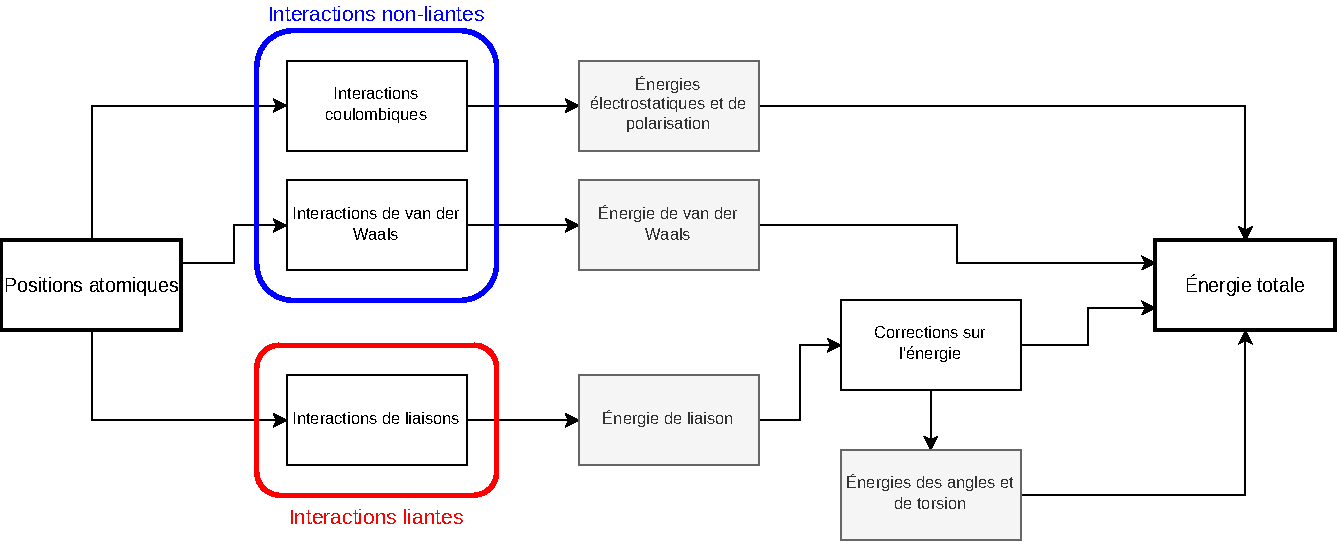
\includegraphics[width=\linewidth]{H2O-ReaxFF-interactions.pdf}
    \caption{Interactions et énergies au sein de \reaxff{} (tiré de \cite{russo_atomistic-scale_2011})}
    \label{fig:interactions_energies_reaxff}
\end{figure}

\reaxff{}\cite{russo_atomistic-scale_2011}\cite{senftle_reaxff_2016} est un potentiel utilisant les ordres de liaison pour modéliser des interactions atomiques en prenant aussi en compte les réactions chimiques (\autoref{fig:interactions_energies_reaxff}).\\
Il a été conçu de façon à obtenir des résultats dont la précision se rapproche des méthodes quantiques, en mettant en jeu autant d'atomes que les méthodes classiques.\\
Enfin, ce potentiel a été comparé à un modèle existant de la molécule d'eau à la \autoref{sec:h2o}.

\textbf{Ordres de liaisons}\\
L'ordre d'une liaison entre un atome $i$ et un atome $j$ est donné par :
\begin{equation}
    BO_{ij}' = \exp \left[p_{bo, 1} \left(\frac{r_{ij}}{r_o}\right)^{p_{bo,2}}\right] + \exp \left[p_{bo,3} \left(\frac{r_{ij}^\pi}{r_o}\right)^{p_{bo,4}}\right] + \exp \left[p_{bo,5} \left(\frac{r_{ij}^{\pi\pi}}{r_o}\right)^{p_{bo,6}}\right]
    \label{eq:ordres_liaisons_reaxff}
\end{equation}
où paramètres $p_{bo,1}, \dots, p_{bo,6}, r_o$ sont des pamramètres issus de calculs \textit{ab initio}, et dépendent de la nature des atomes mis en jeu, et du type de liaison considéré. Les ordres de liaisons sont ensuite corrigés pour être intégrés aux calculs des énergie de liaisons, d'angles et de torsions.

\textbf{Interactions non-liantes}\\
\reaxff{} inclue également les interactions de \vdw{} et \coulomb{} pour \emph{toutes} les paires d'atomes. Les interactions de \vdw{} se basent sur un potentiel de Morse, et ces deux types d'interactions sont protégées par un paramètre $\gamma$ pour éviter de trop grandes attractions et répulsions (\autoref{fig:reaxff_vdw_coulomb}).

\begin{figure}[h!]
    \centering
    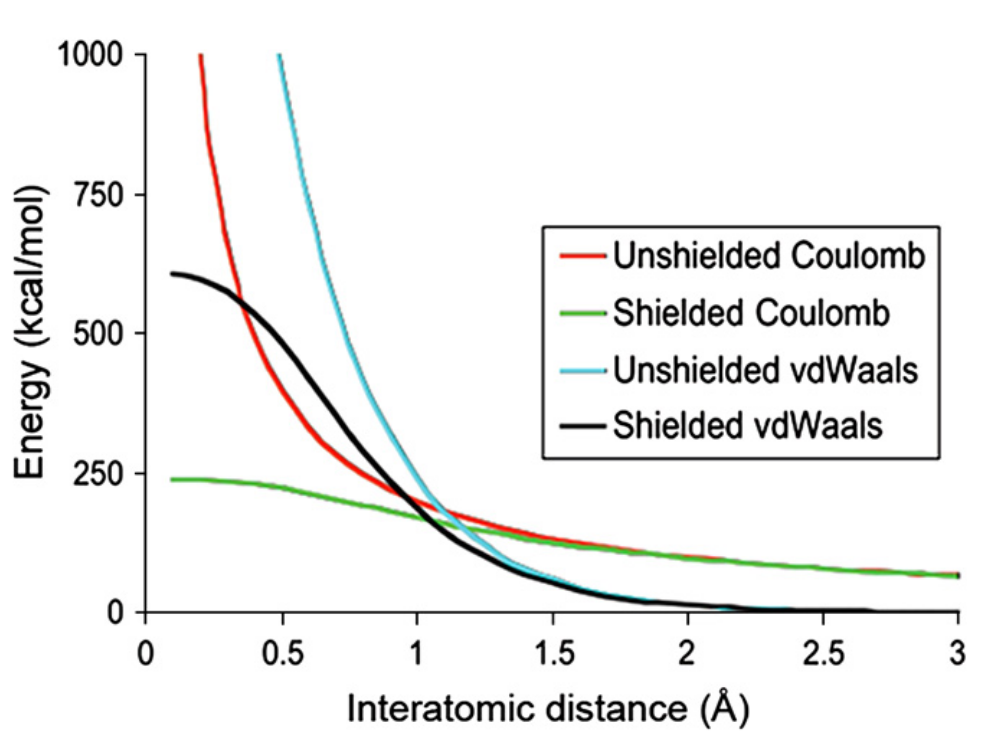
\includegraphics[height = 5 cm]{reaxff_vdw_coulomb.png}
    \caption{Allures des énergies des interactions de \vdw{} et \coulomb{} protégées {\tiny (tiré de \cite{russo_atomistic-scale_2011})}}
    \label{fig:reaxff_vdw_coulomb}
\end{figure}

\textbf{Équilibration des charges}\\
\reaxff{} utilise une méthode d'équilibration des charges, effectuée à chaque pas de temps, basée sur l'\emph{Electron Equilibration Method} (abrégé \eem{})\cite{mortier_electronegativity-equalization_2002} et la méthode \qeq{}\cite{rappe_charge_1991} :
\begin{equation}
    \boxed%
    {
    \frac{\partial E}{\partial q_i} = \chi_i + 2 q_i \eta_i + C \sum_{j = 1}^{n} \frac{q_j}{\left(r_{ij}^3 + (1 / \gamma_{ij})^3\right)^{1/3}}
    }
    \ \text{ et } \ 
    \boxed%
    {
        \sum_{i = 1}^{n} q_i = 0
    }
\end{equation}
où $q_i$ est la charge d'un atome $i$, $\chi_i$ son électronégativité, $\eta_i$ sa dureté, $r_{ij}$ est la distance entre un atome $i$ et un atome $j$ et $\gamma_{ij}$ est le paramètre de protection pour la paire $ij$.


% Presenting EChemDID
    \subsection{Présentation d'\echemdid{}} \label{sec:echemdid}
